\section{Controleren op kwaliteitsgebreken}\label{sec:kwaliteitsgebrek}
Waar in hoofdstuk \ref{sec:consistentie} \textit{Object}s centraal stonden, doen we daar hier afstand van: we abstraheren \textit{Object}s weg en concentreren ons in de plaats op \textit{ClassObject}s. We gebruiken het diagram in figuur \ref{fig:diagram-voorbeeld} weer als begeleidend voorbeeld. In de volgende subsecties overlopen we hoe we de theorie die we gebruiken voor dit probleem opbouwen.

\subsection{Gebruikte logische types en predikaten}
We bewaren het logisch type \textit{ClassObject} en het predikaat \textit{IsSupertypeOf(ClassObject,\\ClassObject)} exact zoals ze zijn in hoofdstuk \ref{sec:consistentie} (en berekenen de transitieve sluiting horende bij \textit{IsSupertypeOf$\backslash2$} op dezelfde manier) en gebruiken daar bijkomend volgende predikaten:

\begin{itemize}
	\item \textbf{\textit{BiAssoc(ClassObject,ClassObject)}}: drukt uit dat er een binaire associatie bestaat tussen de twee klasses.
	\item \textbf{\textit{BiAssocLow(ClassObject,ClassObject,ClassObject,nat)}}: voor \textit{BiAssocLow(x,y,x,n1)} geldt dat voor de binaire associatie tussen klasse \textit{x} en klasse \textit{y} de ondergrens voor de multipliciteit aan de \textit{x}-kant gelijk is aan \textit{n1}; een gelijkaardige interpretatie geldt voor \textit{BiAssocLow(x,y,y,n2)}.
	\item \textbf{\textit{BiAssocHigh(ClassObject,ClassObject,ClassObject,nat)}}: gelijkaardig aan \textit{BiAssocLow$\backslash4$}, maar dan voor de bovengrens van de multipliciteit.
\end{itemize}

Deze predikaten worden ingevuld met een lijst van feiten die af te lezen zijn van het diagram. In hoofdstuk \ref{sec:rol-idp} wordt de logische theorie die het resultaat is van dit proces weergegeven.

\subsection{Kwaliteitsgebreken detecteren}
Er zijn drie kwaliteitsgebreken waarnaar wordt gezocht in de resulterende theorie:

\begin{itemize}
	\item \textbf{Many-to-many associaties}: Dit zijn associaties waar dat de bovengrens van de multipliciteiten aan beide kanten gelijk is aan $*$. Het voorkomen van een many-to-many associatie is doorgaans een teken dat er een klasse ontbreekt in het ontwerp. Het is dus van groot belang dat dit wordt opgespoord en opgelost.
	
	\item \textbf{Losstaande klasse}: Concreet is een losstaande klasse een klasse die geen associatie heeft met een andere klasse in het ontwerp. Zulk een klasse is nutteloos en moet ofwel verbonden worden met een andere klasse of verwijderd worden.
	
	\item \textbf{Overbodige associaties in een klassehi\"erarchie}: Beschouw figuur \ref{fig:hierarchie}. Daar is te zien dat de grenzen van de multipliciteiten in de associatie \textit{Alice}---\textit{Charlie} strengere voorwaarden opleggen dan die van de associatie \textit{Bob}---\textit{David}, en dat daarom de associatie \textit{Bob}---\textit{David} overbodig is. Om de verstaanbaarheid van het diagram te verbeteren, wordt die associatie best verwijderd.
\end{itemize}

We defini\"eren deze respectievelijke gebreken in de logische theorie door middel van de volgende logische zinnen:

\begin{align*}
	\forall{x}[ClassObject]\forall{y}[ClassObject](ManyToMany(x,y) \Leftrightarrow BiAssoc(x,y) \land \\ \lnot\exists{z}[nat](BiAssocHigh(x,y,x,z)) \land \lnot\exists{z}[nat](BiAssocHigh(x,y,y,z)))
\end{align*}

\begin{align*}
	\forall{x}[ClassObject](LooseClass(x) \Leftrightarrow \lnot(\exists{y}[ClassObject](BiAssoc(x,y)) \\ \lor \exists{s}[ClassObject]\exists{y}[ClassObject](IsSupertypeOf(s,y) \land BiAssoc(s,x)))
\end{align*}

\todo{oplossing vinden voor de derde: gewoon verwijzen naar IDP-bestand?}

\begin{figure}
	\label{fig:hierarchie}
	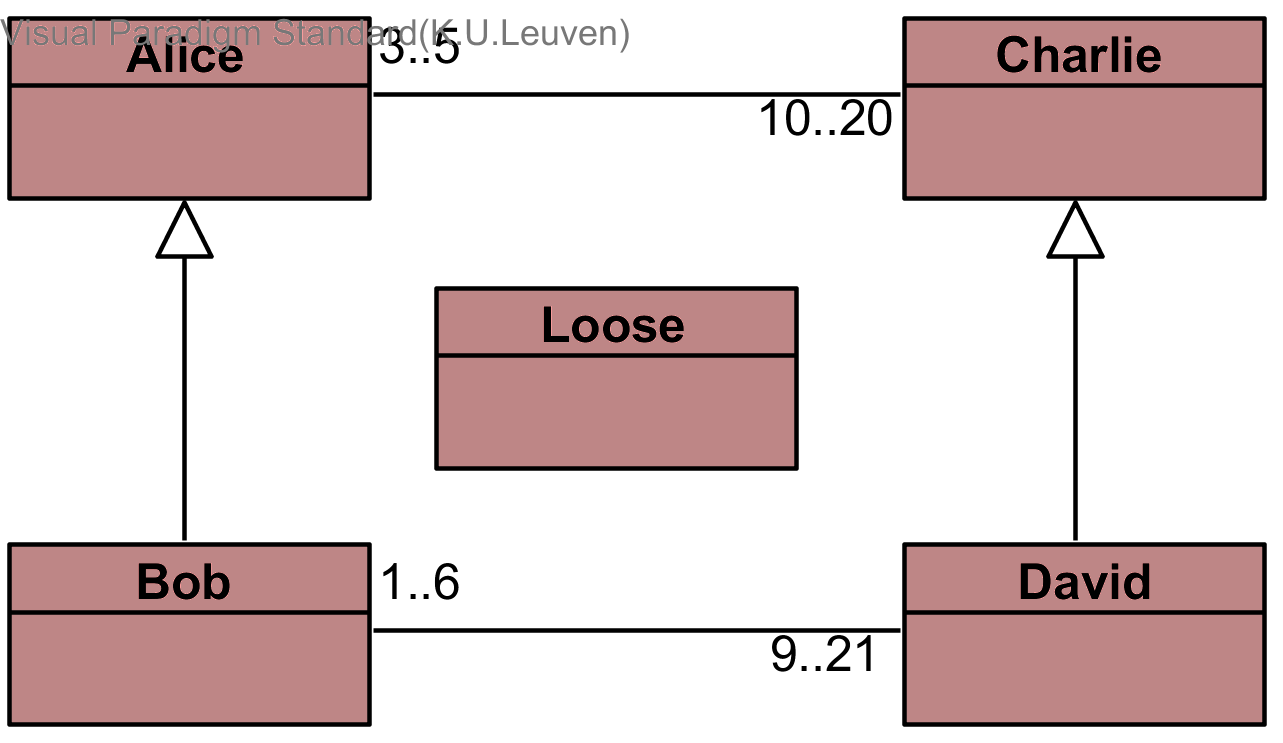
\includegraphics{chap-kwaliteitsgebrek/hierarchy.png}
	\caption{Voorbeeld van meer permissieve multipliciteiten in een klassehi\"erarchie en van een losstaande klasse (zijnde \textit{Loose})}
\end{figure}

Deze regels worden meteen toegevoegd aan de theorie die wordt gegenereerd zoals uitgelijnd eerder in dit hoofdstuk. In hoofdstuk \ref{sec:rol-idp} wordt uitgelegd hoe deze theorie wordt gebruik om kwaliteitsgebreken te vinden.